\begin{figure}
	\centering
	\begin{subfigure}[b]{0.45\linewidth}
		\centering
		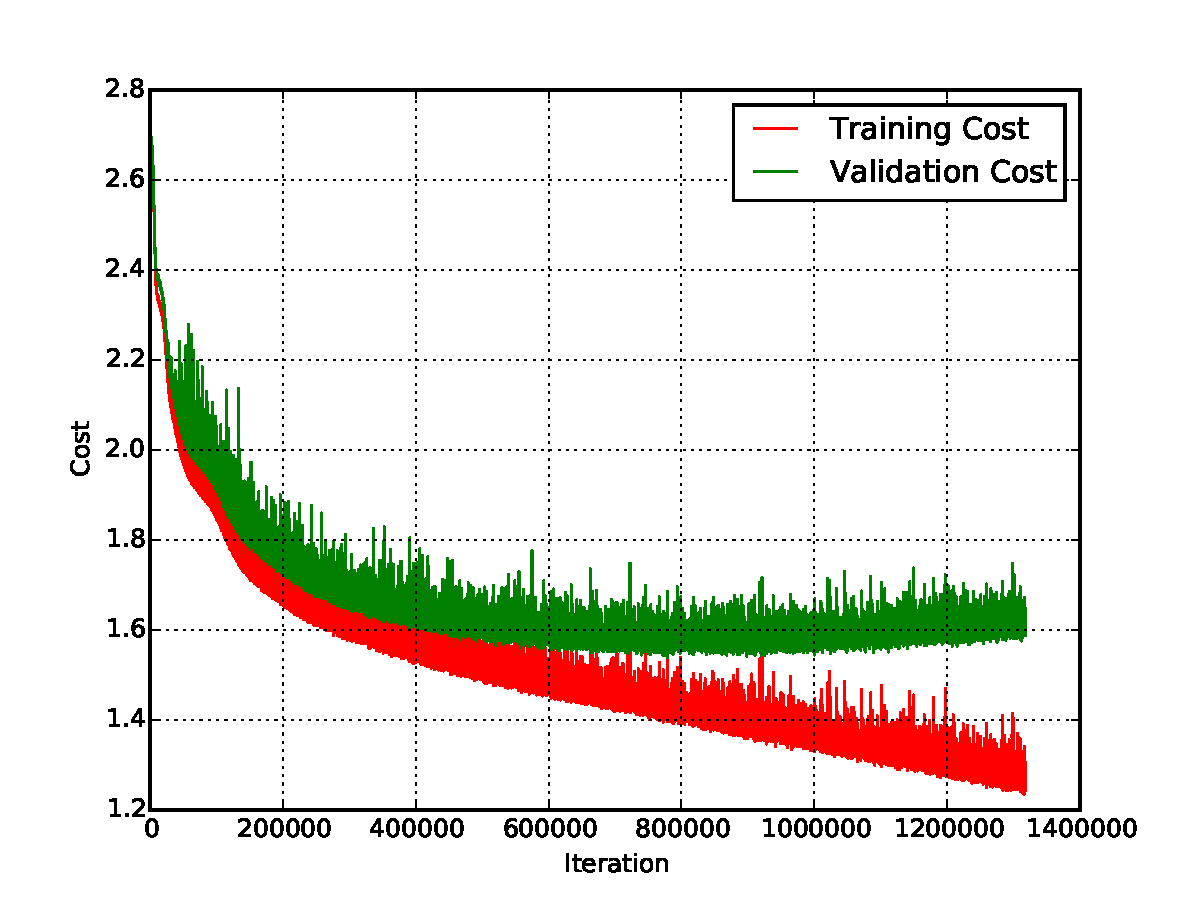
\includegraphics[width=\linewidth]{images/2/train_val_cost.pdf}
		\caption{Training versus Validation Cost}
	\end{subfigure}
	\hfill
	\begin{subfigure}[b]{0.45\linewidth}
		\centering
		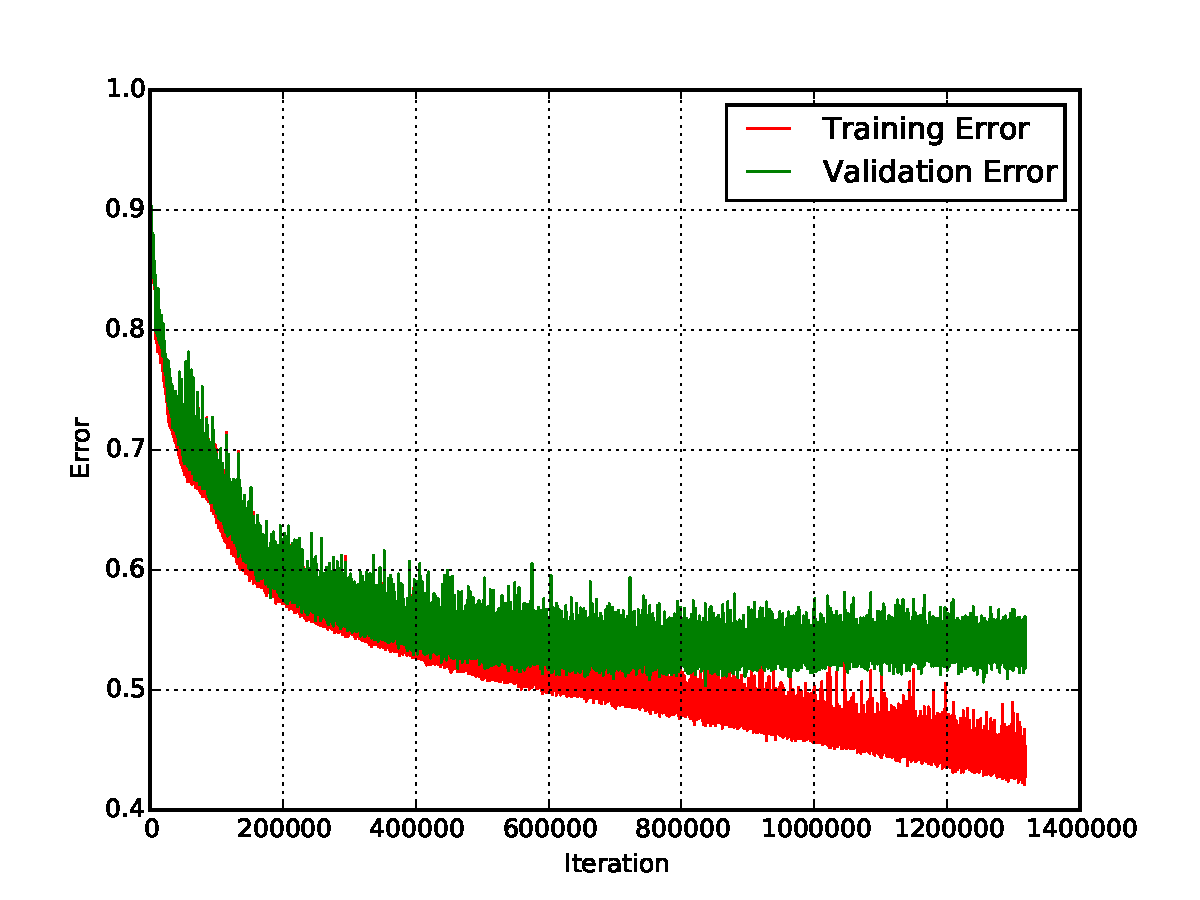
\includegraphics[width=\linewidth]{images/2/train_val_error.pdf}
		\caption{Training versus Validation Error}
	\end{subfigure}
	\caption{Learning curves for a feed-forward neural network with three hidden layers of 256, 128, 64 units trained on LBP.} 
	\label{shrine2_curves}
\end{figure}
\begin{figure}
	\centering
	\begin{subfigure}[b]{0.45\linewidth}
		\centering
		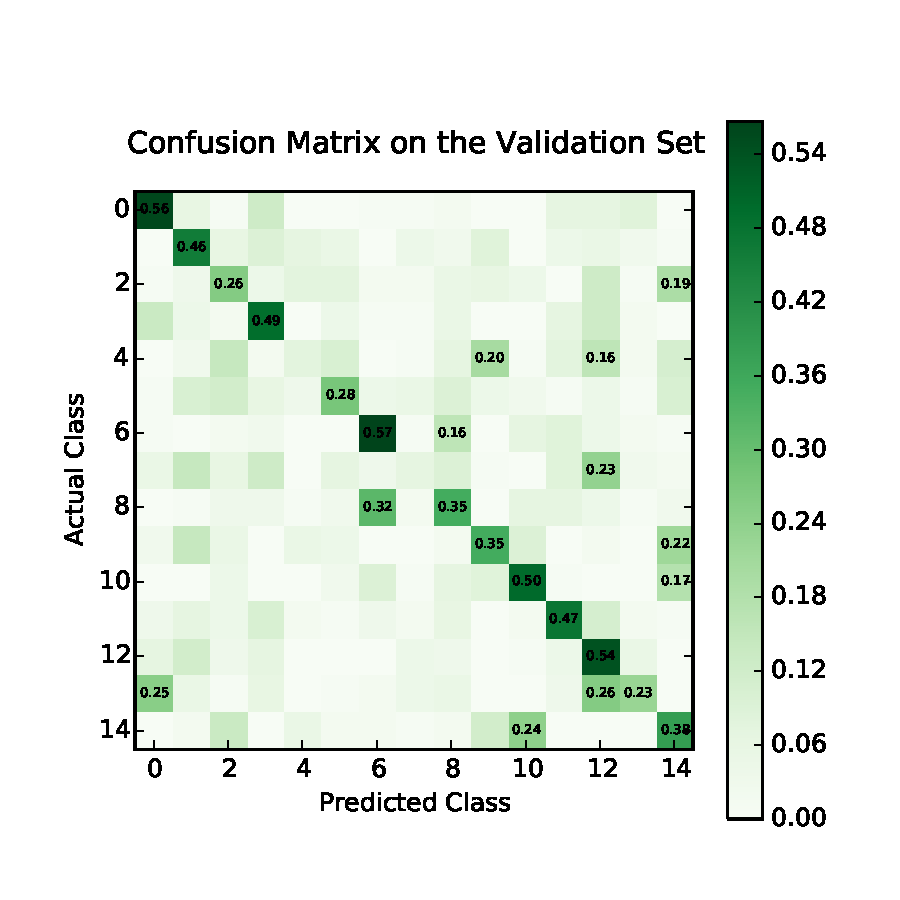
\includegraphics[width=\linewidth]{images/2/cm_valid.pdf}
		\caption{Confusion Matrix on the Validation Set}
	\end{subfigure}
	\hfill
	\begin{subfigure}[b]{0.45\linewidth}
		\centering
		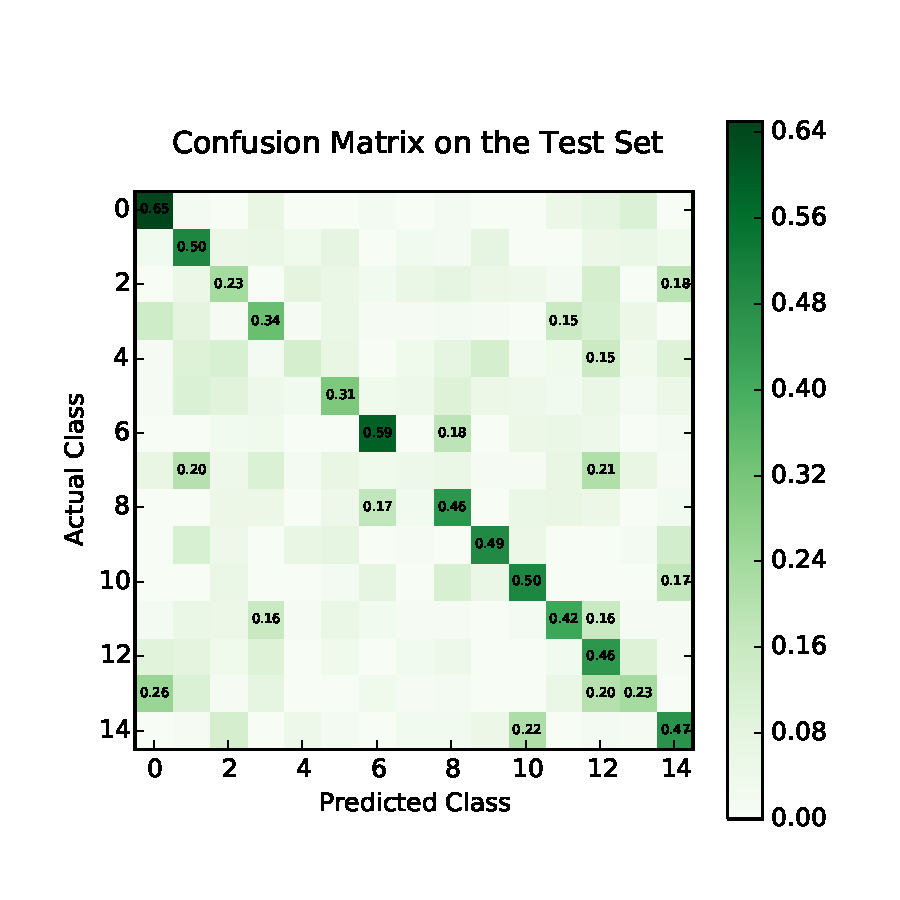
\includegraphics[width=\linewidth]{images/2/cm_test.pdf}
		\caption{Confusion Matrix on the Test Set}
	\end{subfigure}
	\caption{Confusion Matrices for a feed-forward neural network with three hidden layers of 256, 128, 64 units trained on LBP.}
	\label{shrine2_mat}
\end{figure}
